\section{Results}\label{sect:results}
The subvolumes associated with the zonal anatomy in each imaging modality were
measured (Figure~\ref{fig:mr_arfi_volumes}(a)), with moderate correlation
between the ARFI and MR total prostate gland volumes (R$^2$ =
\MRarfiVolTotalRsq), with a mean overestimation of of
\MRarfiVolTotalMeanDiff~$\pm$ \MRarfiVolTotalStdDiff\% by ARFI imaging compared
to MR volumes (Figure~\ref{fig:mr_arfi_volumes}(b)).  Central gland volumes
were well-correlated between ARFI and MR images (R$^2$ = \MRarfiVolCentralRsq)
with no significant mean over/under-estimation (\MRarfiVolCentralMeanDiff~$\pm$
\MRarfiVolCentralStdDiff\%), but significant variability between the cases
(Figure~\ref{fig:mr_arfi_volumes}(c)).  Table~\ref{tab:mr_arfi_volumes} has the
individually-measured volumes for MR and ARFI imaging for each study subject.

\begin{figure}[htb!]
\centering
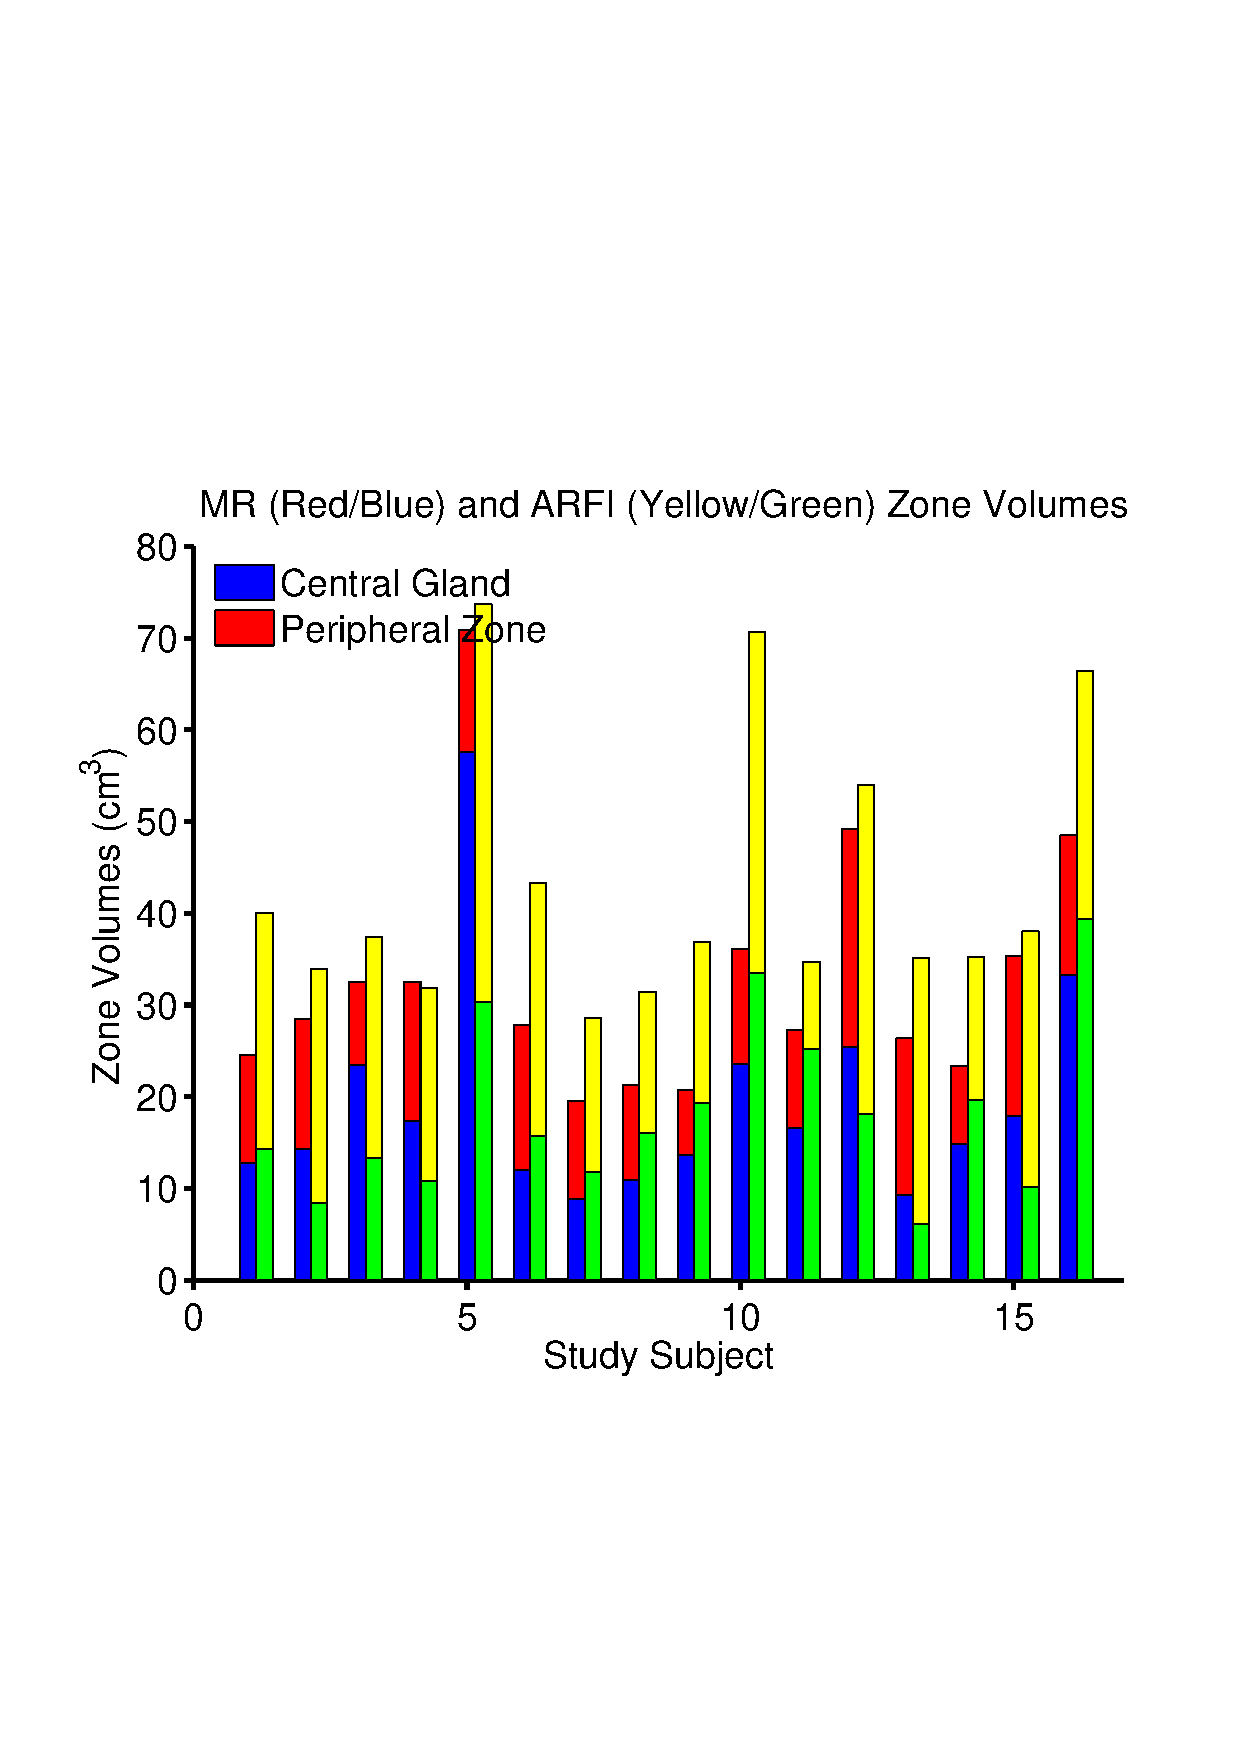
\includegraphics[width=0.5\linewidth]{figs/mr_arfi_volumes.pdf}
\caption{MR and ARFI volumes - need more text here}
\label{fig:mr_arfi_volumes} 
\end{figure}


Weights and axis measurements from the gross pathology processing of the
excised prostates were collected (Table~\ref{tab:path_data}), and using the
axis measurements (lateral-to-lateral, anterior-to-posterior, and
apex-to-base), the prostate volume was approximated as a tri-axial ellipsoid,
and its volume was estimated (\ref{eqn:ellipsoid_volume}).  Prostate weights
were moderately correlated with estimated pathology ellipsoidal prostate
volumes (Figure~\ref{fig:mr_arfi_weight}(a), R$^2$ = \pathVolWeightRsq).  There
was moderate correlation between the prostate weight and the
image-reconstructed prostate volumes (Figure~\ref{fig:mr_arfi_weight}(b), R$^2$
= \weightMRrsq~(MR) and \weightARFIrsq~ (ARFI)), though there was weaker
correlation with the ellipsoidal approximation of the measurement prostate
volume and the image-reconstructed volumes (Figure~\ref{fig:mr_arfi_weight}(c),
R$^2$ = \pathVolMRrsq~(MR) and \pathVolARFIrsq~(ARFI)).  

\begin{figure}[htb!]
\centering
\begin{tabular}{lll}
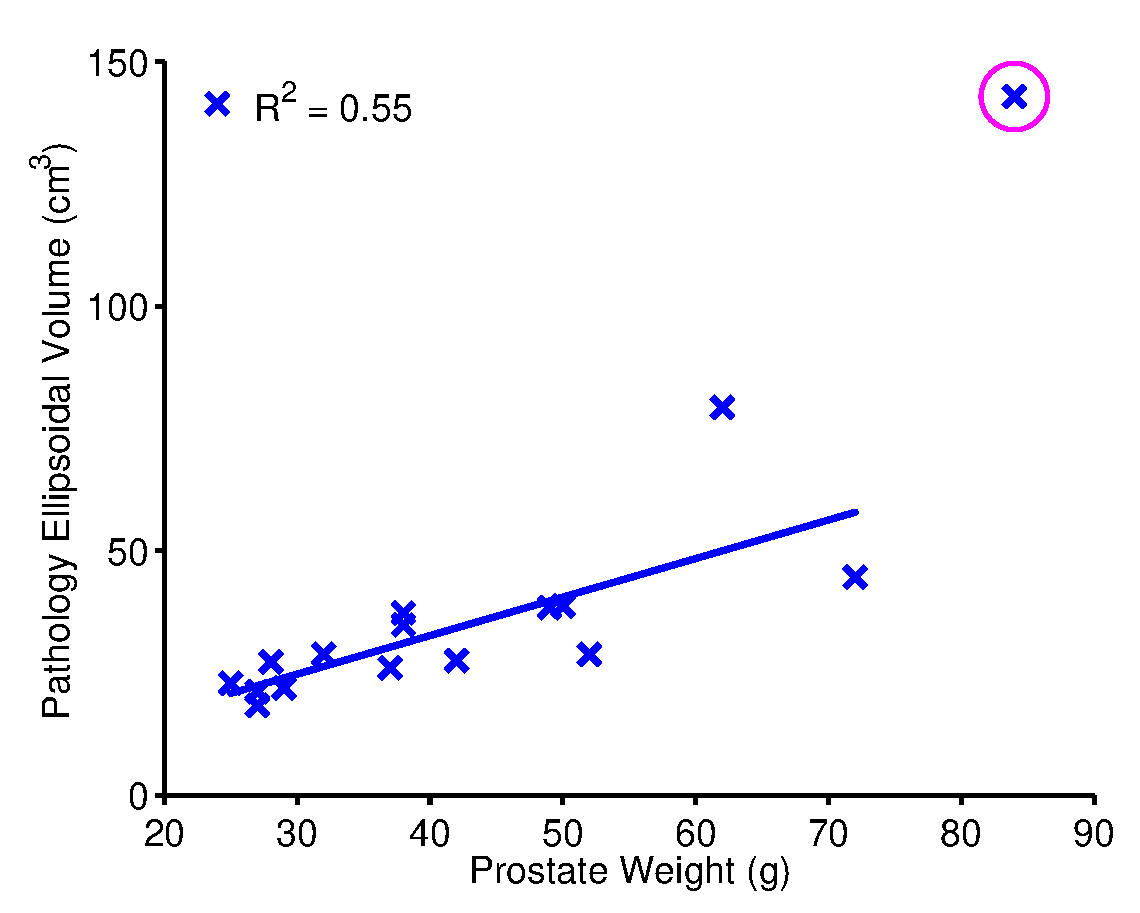
\includegraphics[width=0.3\linewidth]{figs/corr_path_vol_weight_vol} &
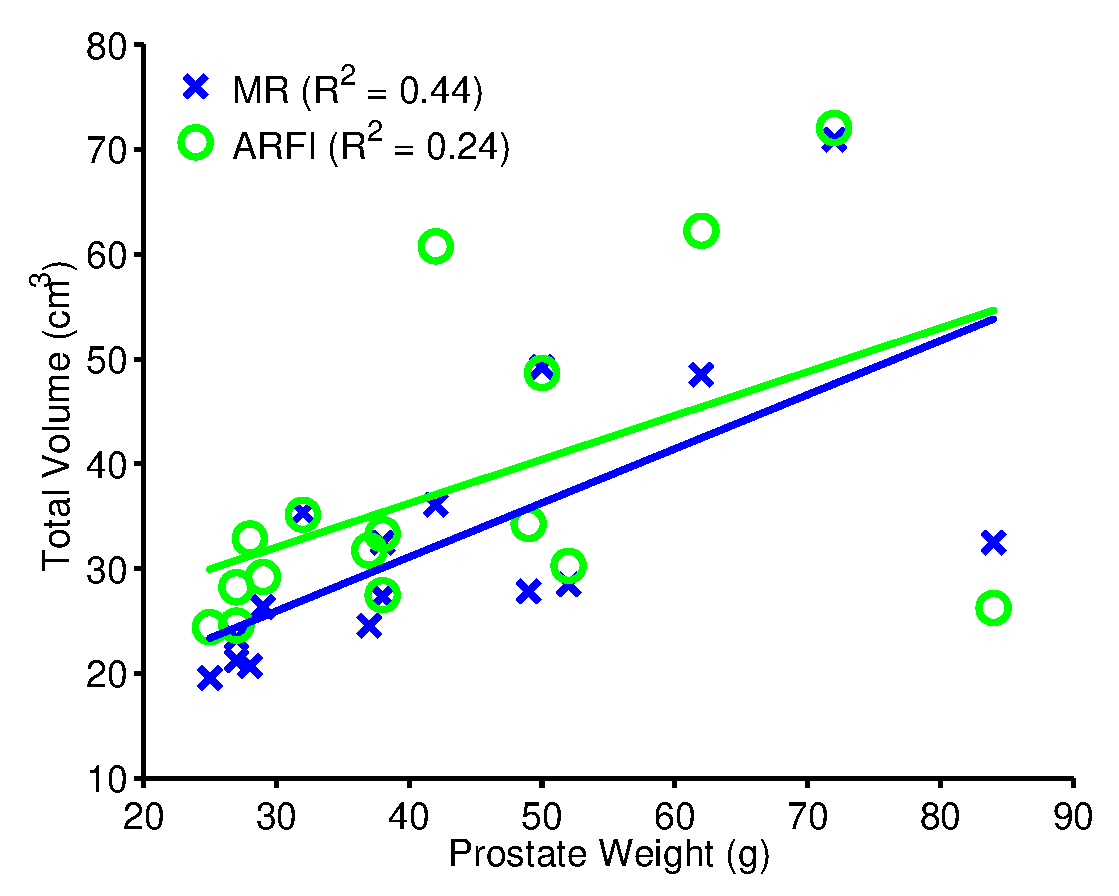
\includegraphics[width=0.3\linewidth]{figs/corr_weight_vol} &
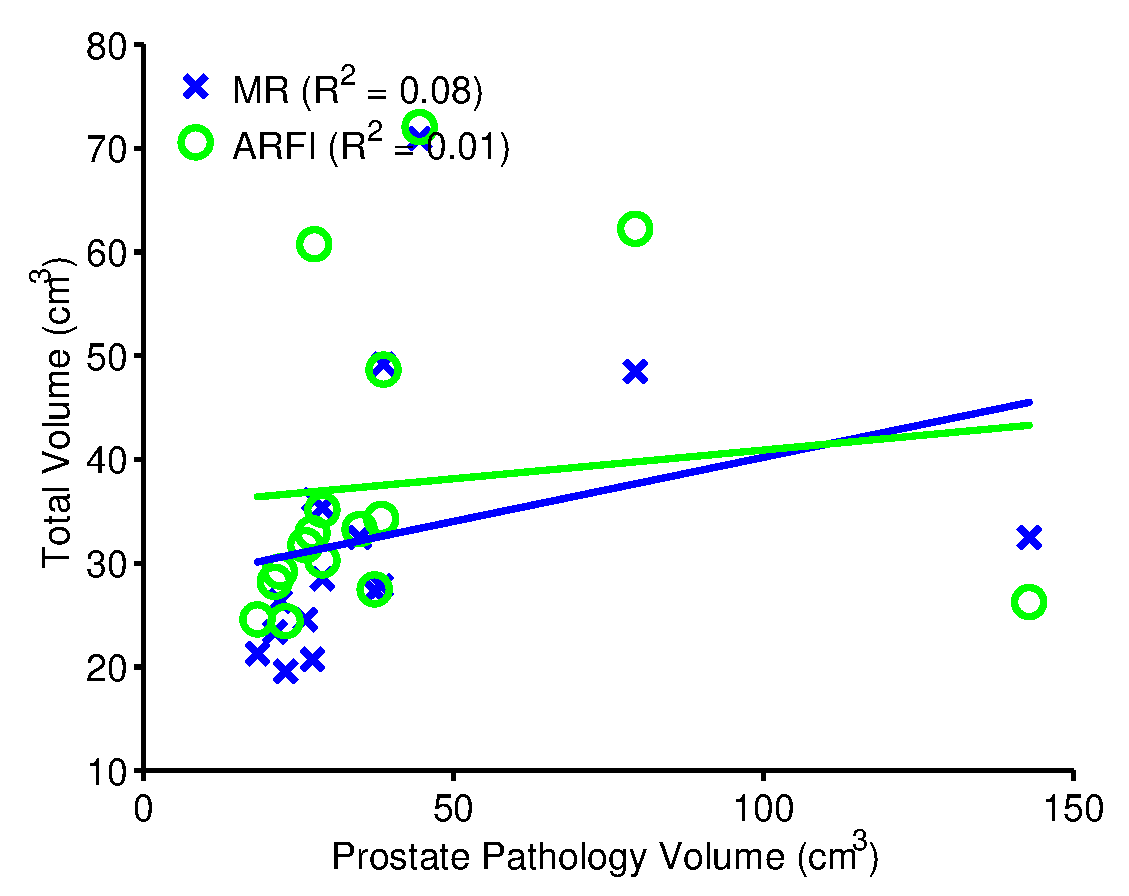
\includegraphics[width=0.3\linewidth]{figs/corr_pathVol_vol} \\
(a) Path Weight : Path Volume & (b) Image Volume : Prostate Weight & (c) Image Volume : Path Volume \\
\end{tabular}
%\begin{tabular}{ll}
%\includegraphics[width=0.3\linewidth]{figs/corr_weight_vol_no4} &
%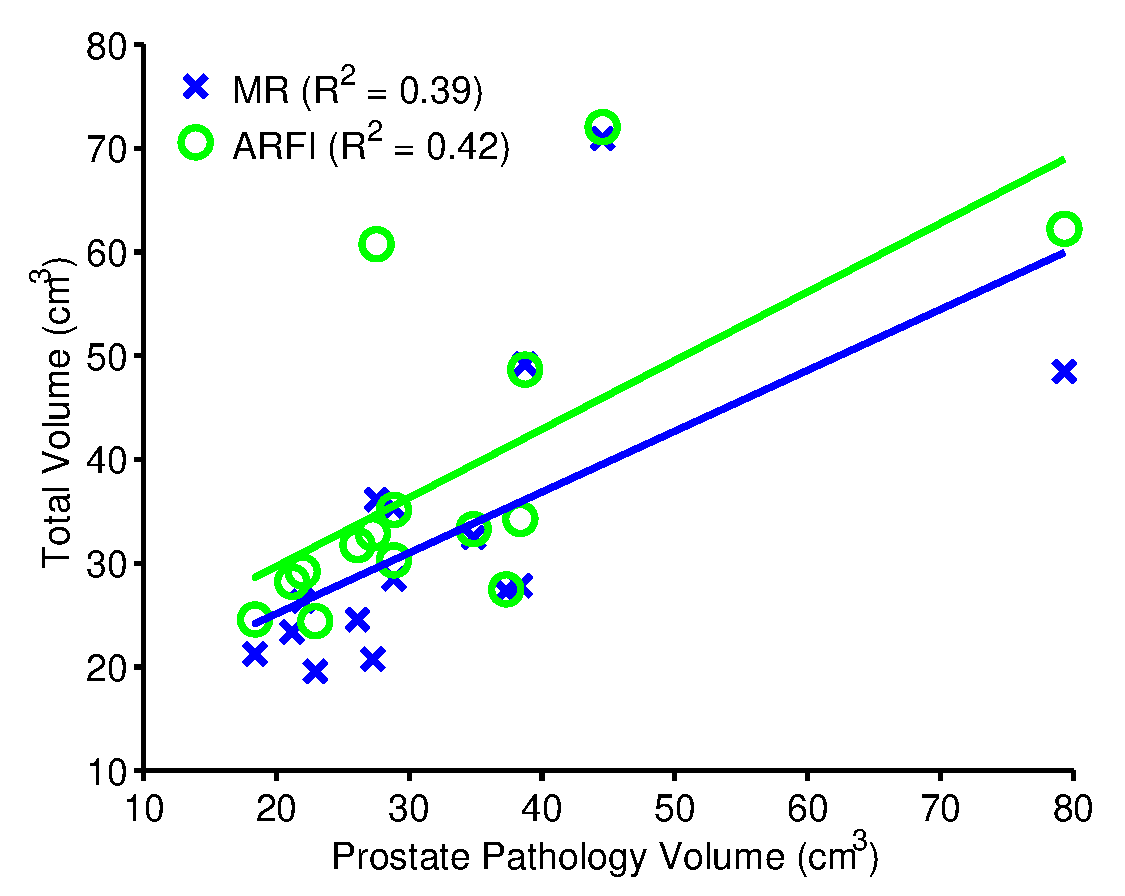
\includegraphics[width=0.3\linewidth]{figs/corr_pathVol_vol_no4} \\
%(d) Image Volume : Prostate Weight (-4) & (e) Image Volume : Path Volume (-4) \\
%\end{tabular}
\caption{Tri-axial pathology measurements were used to make an ellipsoidal
    prostate volume approximation based on gross pathology axis measurements,
    which was moderately well-correlated with the excised prostated weights (a,
    R$^2$ = 0.68).  T2WI MR (blue, X) showed a moderate correlation between the
    reconstructed volumes and prostate weight (R$^2$ = 0.44), while volumes
    reconstructed from ARFI images (green, O) showed weaker correlation (R$^2$
    = 0.21) (b).  Even weaker correlations existed between both T2WI MR and
    ARFI image volumens and approaximated ellipsoidal prostate pathology
    volumes (R$^2$ = 0.08 and 0.01, respectively) (c).  It should be noted in
    these figures that two study subjects had excessively large prostates that
    were difficult to fully capture in imaging (volumes $>$ 60 cm$^3$),
    especially in their anterior region, and they were, therefore, grossly
    underestimated in size.}
\label{fig:mr_arfi_weight}
\end{figure}


Measurements of the prostate total gland and CG dimensions along the three
standard anatomic axes (apex-to-base, lateral-to-lateral, and
anterior-to-posterior) were made (Table~\ref{tab:mr_arfi_axes}), and the
correlation between the imaging axis measurements was analyzed
(Figure~\ref{fig:mr_arfi_path_axes}).  ARFI was most correlated to MR in the
lateral-to-lateral axis in both the total gland and CG (R$^2$ =
\totalLatLatRsq~and \centralLatLatRsq, respectively), with mean overestimates
of \ARFImrTotalLatLatMeanPct~$\pm$ \ARFImrTotalLatLatStdPct\%~and
\ARFImrCentralLatLatMeanPct~$\pm$ \ARFImrCentralLatLatStdPct\%, respectively
(Table~\ref{tab:mr_arfi_axes_error}).  ARFI had moderate correlation with the
total prostate gland and CG axes in the anterior-to-posterior dimension (R$^2$
= \totalAntPostRsq~and \centralAntPostRsq), respectively, with differences of
\ARFImrTotalAntPostMeanPct~$\pm$ \ARFImrTotalAntPostStdPct\% and
\ARFImrCentralAntPostMeanPct~$\pm$ \ARFImrCentralAntPostStdPct\%.  ARFI imaging
had weak correlation with MR images in the apex-to-base dimension (R$^2$ =
\totalApexBaseRsq, total gland and R$^2$ = \centralApexBaseRsq, CG), with
underestimates of \ARFImrTotalApexBaseMeanPct~$\pm$
\ARFImrTotalApexBaseStdPct\% and \ARFImrCentralApexBaseMeanPct~$\pm$
\ARFImrCentralApexBaseStdPct\%, respectively.

\begin{figure}[htb!]
\centering
\begin{tabular}{ccc}
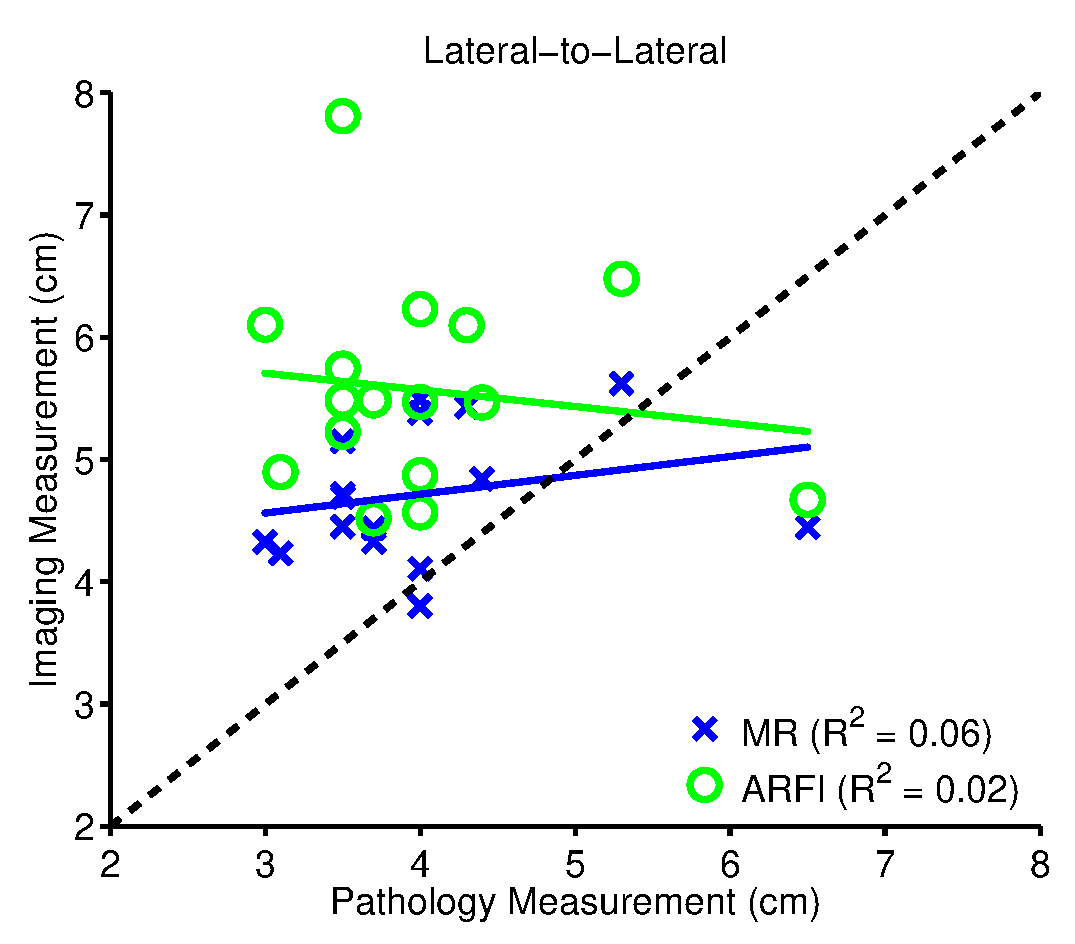
\includegraphics[width=0.3\linewidth]{figs/Lateral-to-Lateral} &
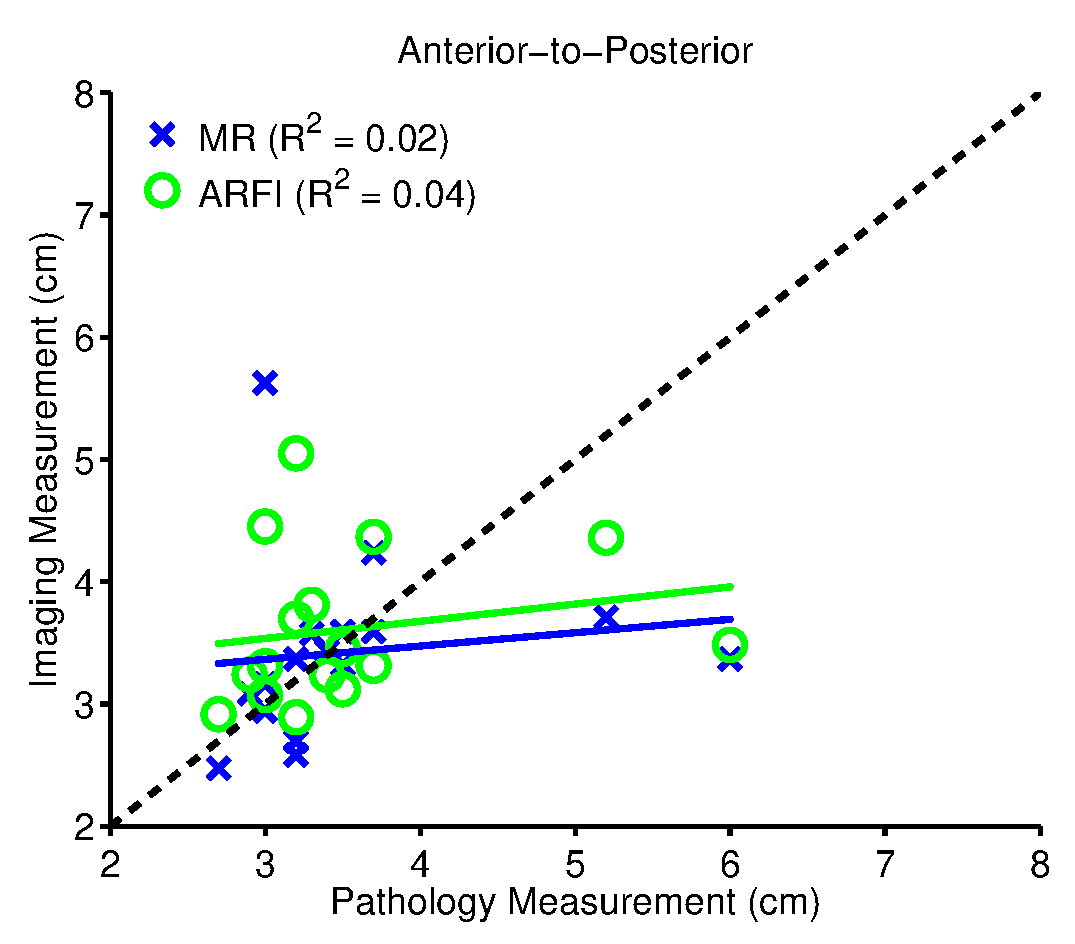
\includegraphics[width=0.3\linewidth]{figs/Anterior-to-Posterior} &
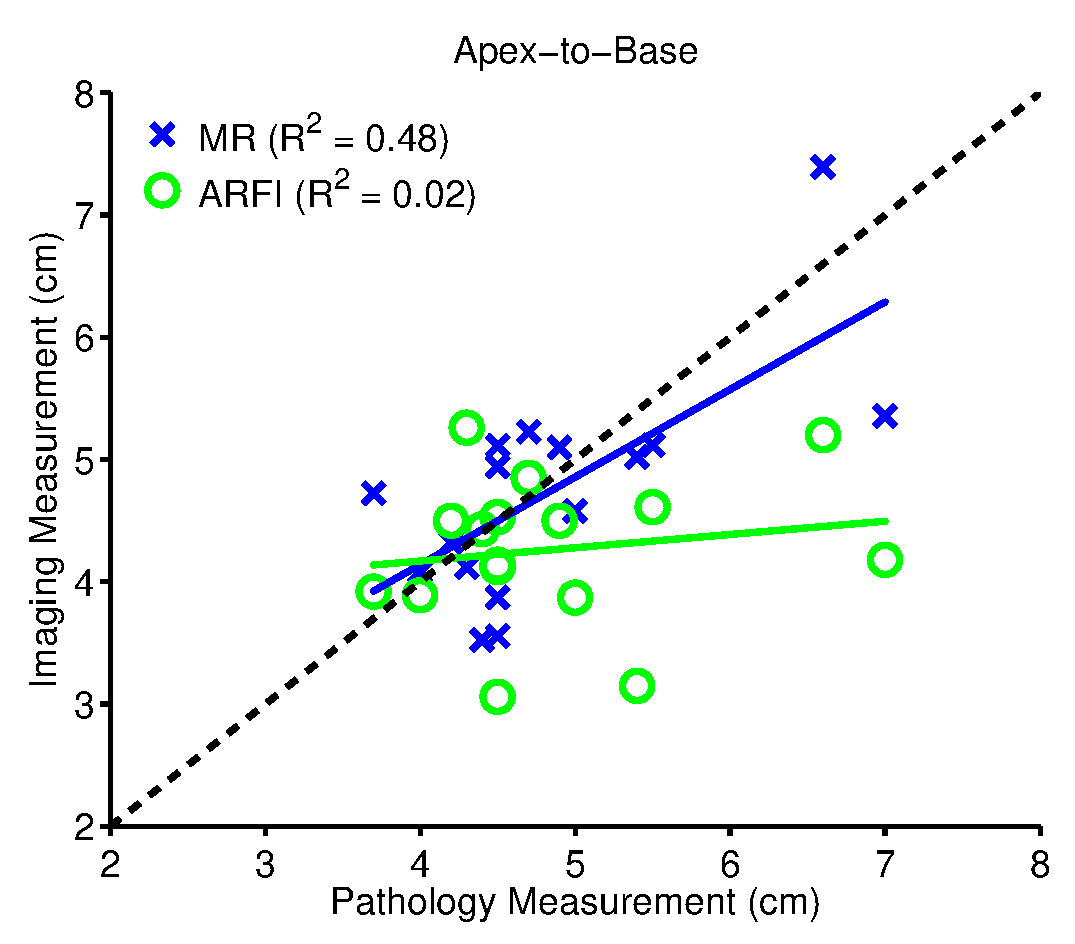
\includegraphics[width=0.3\linewidth]{figs/Apex-to-Base} \\
(a) & (b) & (c) \\
\end{tabular}
\caption{Measurements of the prostate dimensions along the three standard
anatomic axes: lateral-to-lateral (a), anterior-to-posterior (b) and
apex-to-base (c).  The correlation between the imaging axis measurements and
pathology was performed for each orientation.  The black dashed-line represents
the projection of perfectly-correlated measurements between imaging and
patholoy.  Notice that there is no correlation between imaging and pathology in
the lateral-to-lateral and anterior-to-posterior axes, with a general
over-estimation of the lateral-to-lateral axis in the imaging.  The MR
estimation of the apex-to-base dimension showed moderate correlation with
pathology, with the ARFI image apex-to-base approximation having an overall
underestimation in this orientation.  The over-/under-estimation of each imaging modality relative to gross pathology is summarized in Table~\ref{tab:mr_arfi_path_axes}.}
\label{fig:mr_arfi_path_axes} 
\end{figure}


\begin{table}[h!]
\centering
\caption{Difference in ARFI imaging axis measurements relative to MR T2WI measurements.}
\begin{tabular}{|l|l|l|} \hline
 & {\bf ARFI:MR} & {\bf ARFI:MR} \\ 
 & {\bf Total Gland (\%)} & {\bf Central Gland (\%)} \\ \hline 
{\bf Lateral-to-Lateral} & 18.4 $\pm$ 13.9 & 21.5 $\pm$ 14.3 \\ 
{\bf Anterior-to-Posterior} & 7.4 $\pm$ 18 & -0.6 $\pm$ 20.8 \\ 
{\bf Apex-to-Base} & -10.8 $\pm$ 16.8 & -28.8 $\pm$ 9.4 \\ 
\hline
\end{tabular}
\label{tab:mr_arfi_axes_error}
\end{table}


%\begin{figure}[htb!]
\centering
\begin{tabular}{ccc}
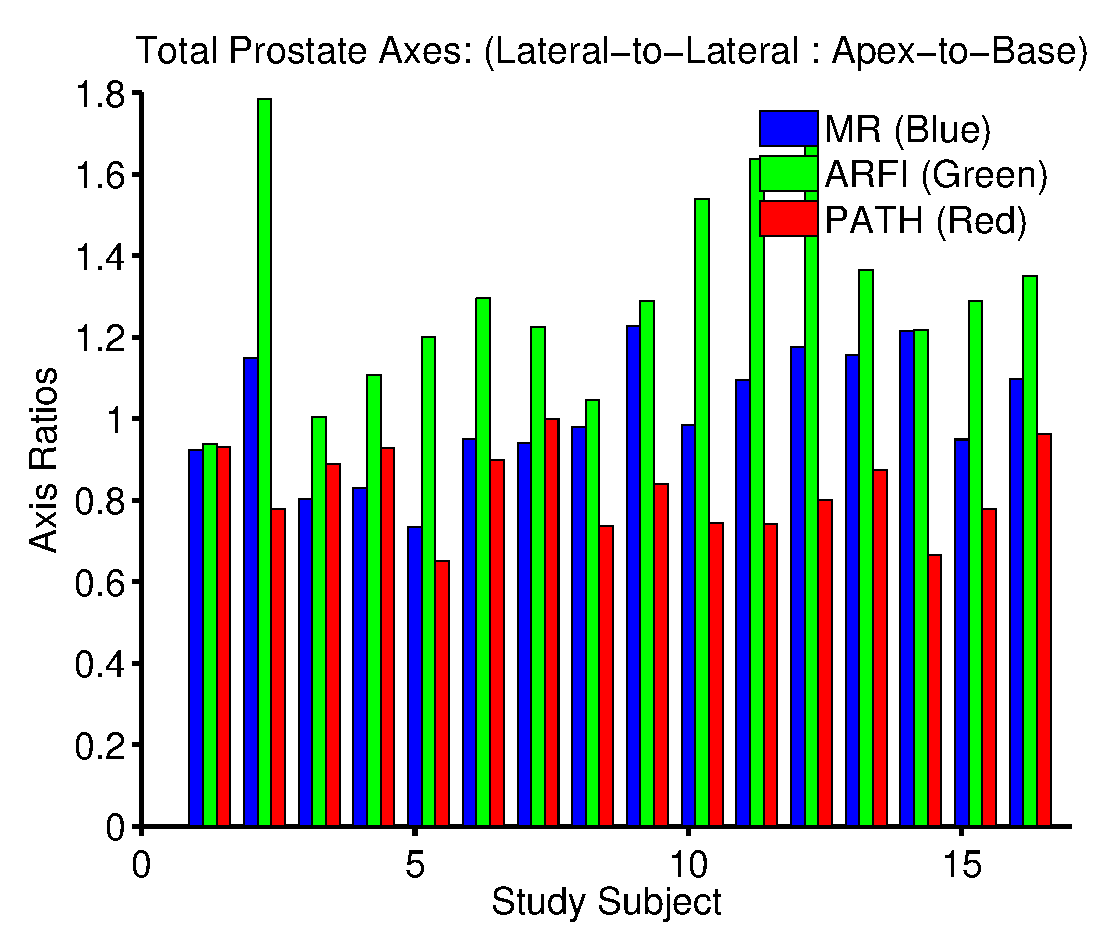
\includegraphics[width=0.3\linewidth]{figs/mr_arfi_total_axes1} &
\includegraphics[width=0.3\linewidth]{figs/mr_arfi_total_axes2} &
\includegraphics[width=0.3\linewidth]{figs/mr_arfi_total_axes3} \\
(a) & (b) & (c) \\
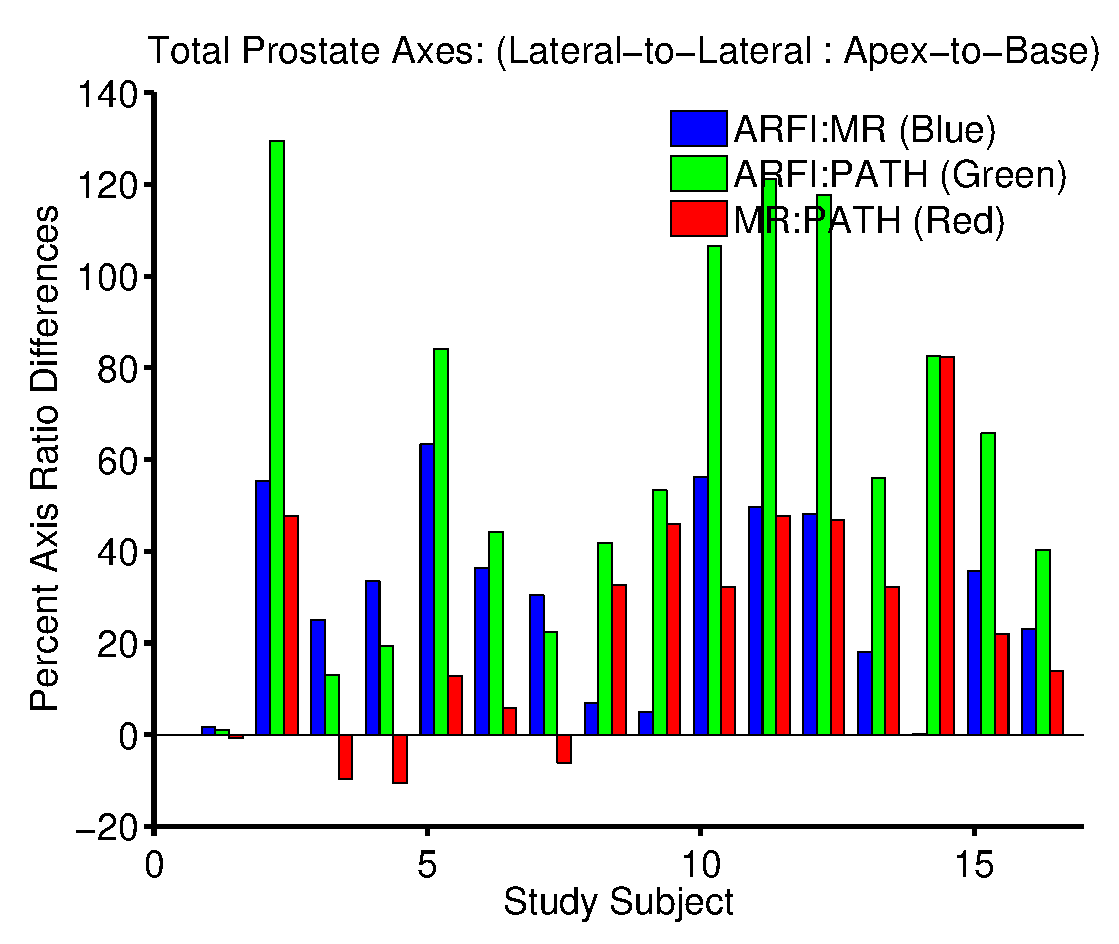
\includegraphics[width=0.3\linewidth]{figs/mr_arfi_total_over_under1} &
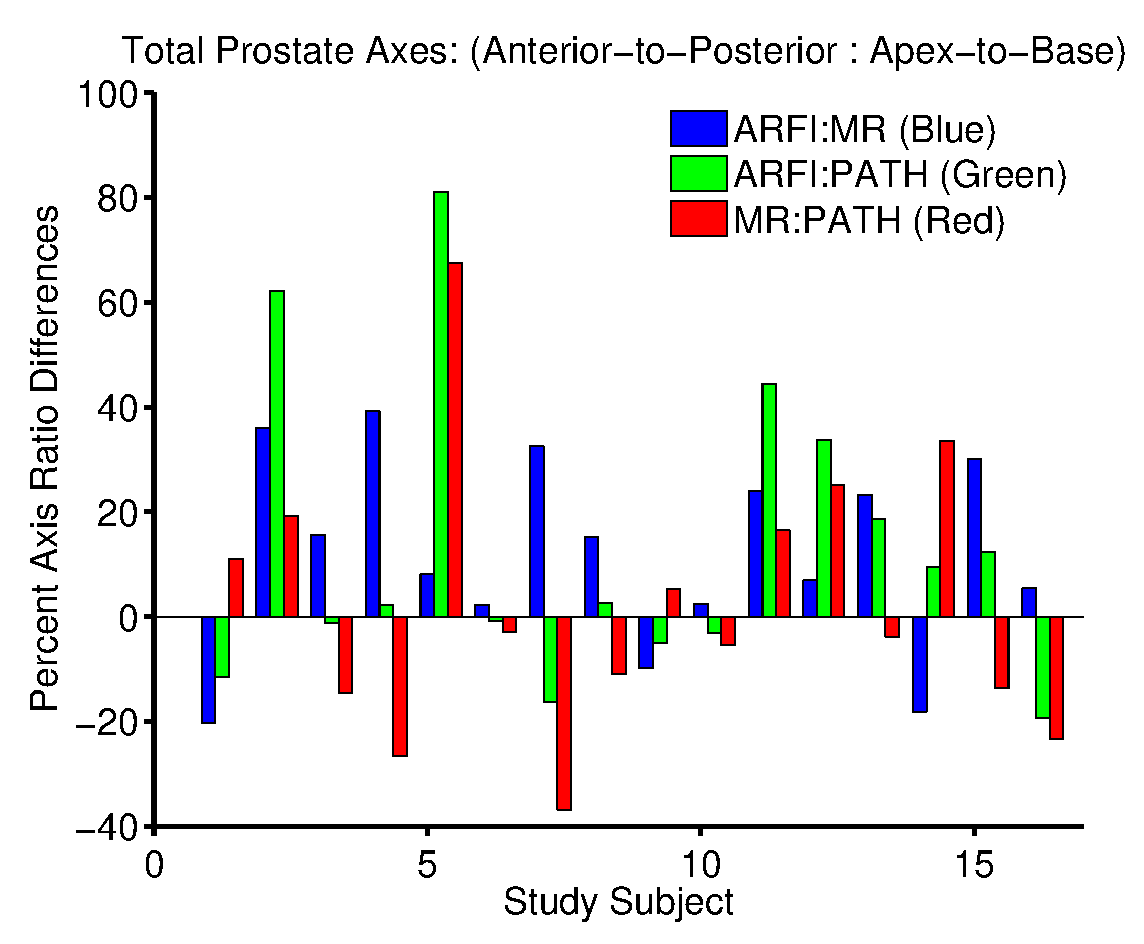
\includegraphics[width=0.3\linewidth]{figs/mr_arfi_total_over_under2} &
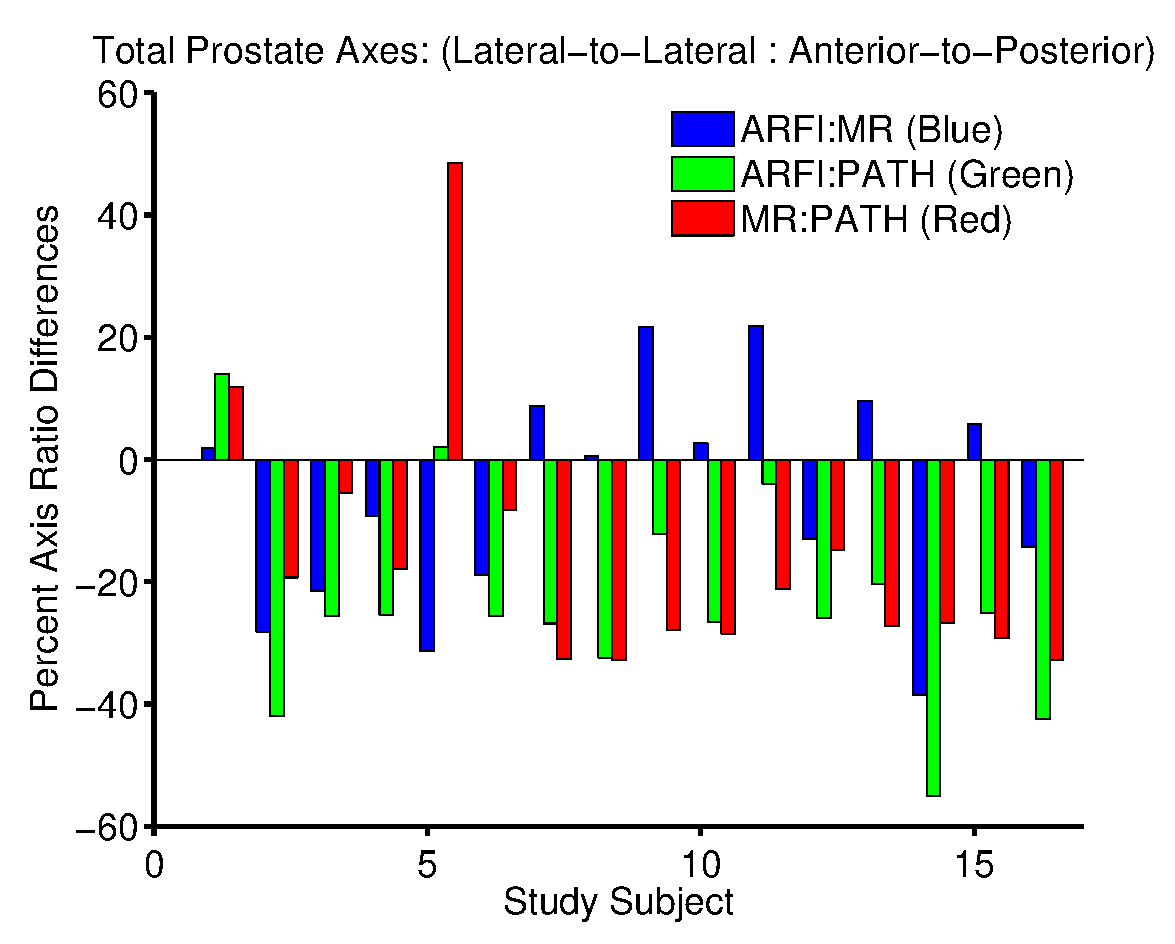
\includegraphics[width=0.3\linewidth]{figs/mr_arfi_total_over_under3} \\
(d) & (e) & (f) \\
\end{tabular}
\caption{Comparison of the ratios of the three anatomic axis measurement ratios
    for T2WI MR (top row, blue), ARFI imaging (top row, green) and gross
    pathology (top row, red).  The over/underestimation of the axis ratios
    between ARFI imaging : T2WI MR : Pathology are shown in the bottom row
    (d-f), with mean ratio differences compiled in
    Table~\ref{tab:axis_ratio_over_under}.}
\label{fig:mr_arfi_total_axes} 
\end{figure}


%\begin{figure}
\centering
\begin{tabular}{ccc}
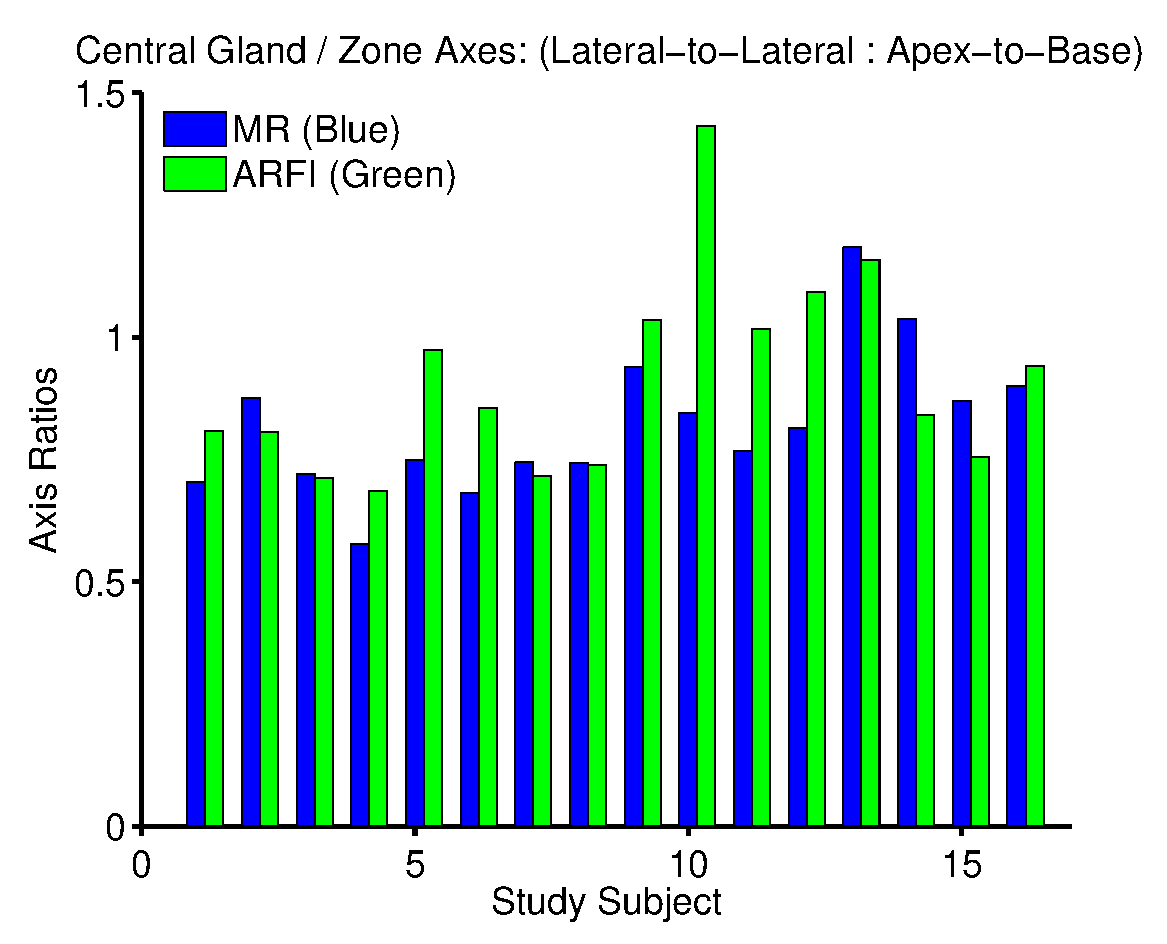
\includegraphics[width=0.3\linewidth]{figs/mr_arfi_central_axes1} &
\includegraphics[width=0.3\linewidth]{figs/mr_arfi_central_axes2} &
\includegraphics[width=0.3\linewidth]{figs/mr_arfi_central_axes3} \\
(a) & (b) & (c) \\
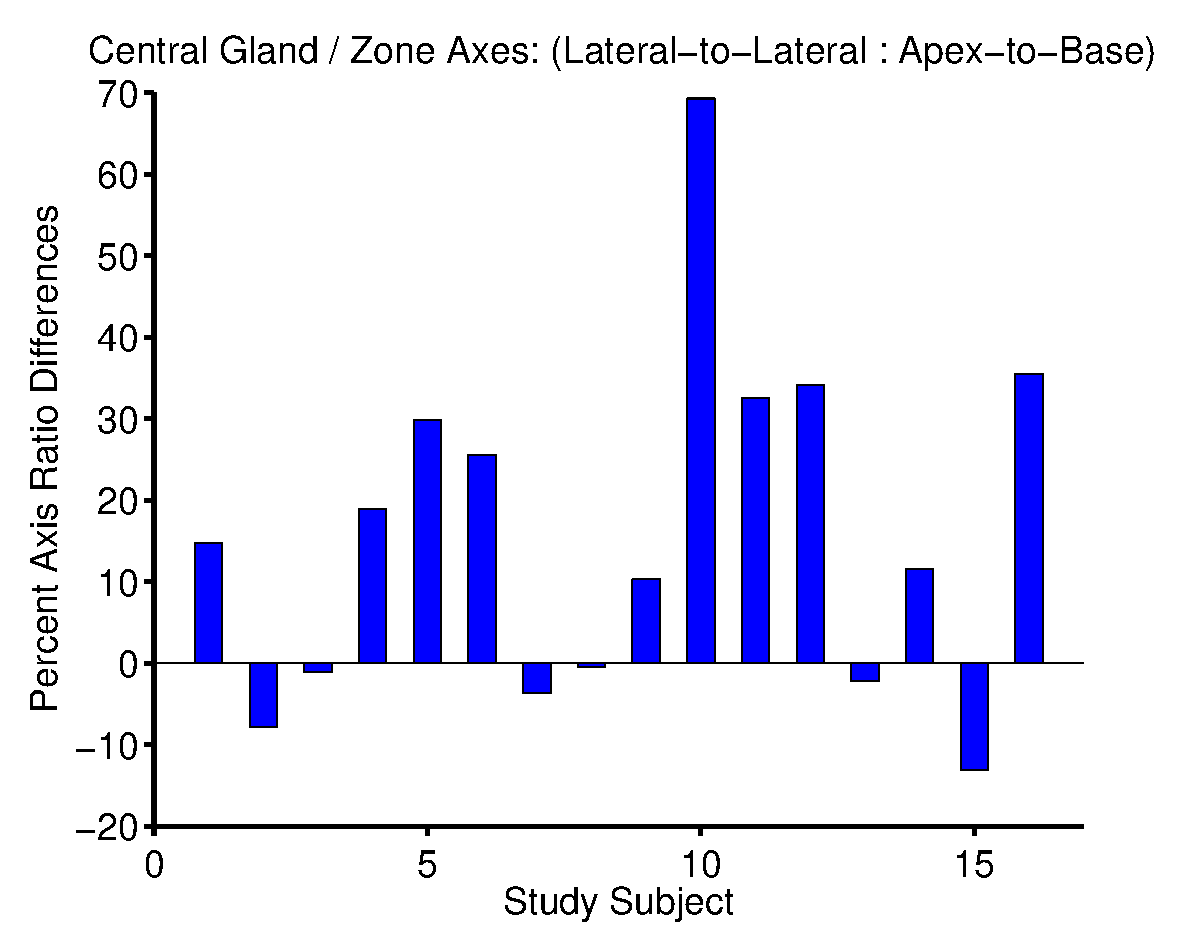
\includegraphics[width=0.3\linewidth]{figs/mr_arfi_central_over_under1.eps} &
\includegraphics[width=0.3\linewidth]{figs/mr_arfi_central_over_under2.eps} &
\includegraphics[width=0.3\linewidth]{figs/mr_arfi_central_over_under3.eps} \\
(a) & (b) & (c) \\
\end{tabular}
\caption{Comparison of the ratios of the three anatomic axis measurement ratios
    for T2WI MR (top row, blue) and ARFI imaging (top row, green).  The
    over/underestimation of the axis ratios between ARFI imaging and T2WI MR
    are shown in the bottom row (d-f), with mean ratio differences compiled in
    Table~\ref{tab:axis_ratio_over_under}.}
\label{fig:mr_arfi_central_axes} 
\end{figure}


%\begin{table}
\centering
\caption{Mean axis ratio differences between ARFI imaging, T2WI MR and
    pathology for the total prostate volume and central gland / zone for the
    imaging modalities.  The three axis ratios analyzed were:
    lateral-to-lateral : apex-to-base (LL:AB), anterior-to-posterior :
    apex-to-base (AP:AB), and lateral-to-lateral : anterior-to-posterior
    (LL:AP).}
\begin{tabular}{|l|l|l|l|l|} \hline
{\bf Image Modality} & {\bf Comparative Measure} & {\bf Total / Central} & {\bf Axes} & {\bf Axis Ratio Difference (\%)} \\ \hline
ARFI & MR & Total & LL:AB & 13.9 $\pm$ 22.9 \\ 
ARFI & PATH & Total & LL:AB & 39.3 $\pm$  27.6 \\ 
MR & PATH & Total & LL:AB & 24.7 $\pm$ 26.0 \\ 
ARFI & MR & Total & AP:AB & 5.2 $\pm$ 22.6 \\ 
ARFI & PATH & Total & AP:AB & 5.4 $\pm$  28.3 \\ 
MR & PATH & Total & AP:AB & 2.5 $\pm$ 26.0 \\ 
ARFI & MR & Total & LL:AP & -6.4 $\pm$ 18.3 \\ 
ARFI & PATH & Total & LL:AP & -23.3 $\pm$  17.1 \\ 
MR & PATH & Total & LL:AP & -16.5 $\pm$ 21.1 \\ 
ARFI & MR & Central & LL:AB & 12.0 $\pm$ 22.5 \\ 
ARFI & MR & Central & AP:AB & -8.8 $\pm$ 20.8 \\ 
ARFI & MR & Central & LL:AP & -15.4 $\pm$ 25.9 \\ 

\hline
\end{tabular}
\label{tab:axis_ratio_over_under}
\end{table}

